\chapter{QCA Defects Simulator}
\label{QCA_Defects_Simulator}

This chapter introduces the QCA Defects Simulator developed in this work, which is based on a novel methodology for analysis of errors related to defective cells or phase-shifted clock signals. The tool QCADesigner version 2.0.3 is extended by a defects simulation module in order to provide support to an automatic process for evaluation of the structures, which provides the error-free simulations rate and the design heat map as the output data.

The remaining contents of the chapter is divided into three main subsections. The first one refers to the introduction of the novel methodology for defects insertion and error analysis for QCA. The intermediate subsection describes the defects simulation module that is implemented as an extension for the tool QCADesigner. At last, the third part of this chapter introduces the means by which the output data is presented.

\section{Methodology}

The majority of the error analysis methods already reported in the literature for the QCA paradigm proceed to the manual defect insertion, such as in \cite{tahoori04} \cite{dai10} and \cite{yang12}. Nevertheless, there are some approaches that enable the defect insertion and results analysis through automatic process, as described in \cite{armstrong03}, \citeonline{schulhof07}, \cite{khatun06} and \cite{karim09}. However, almost all automatic methods reported are not enough flexible to allow the insertion of multiple defect classes into the cells in a same structure at the same time. Moreover, the error analysis approaches usually use fixed parameters for the defects value, as the displacement/misalignment shifts, rotation angles and the number of extra/missing dots in a cell \cite{tahoori04}, \cite{dai10} and \cite{yang12}. A most complete approach for error analysis for QCA structures is reported in \cite{armstrong03}. It allows a flexible defects insertion by means of probability values and further settings. The more detailed description of the method may be found in the Section \ref{subsection:review_methodologies_structures}. However, the paper does not report any results.

This work introduces a novel simulation-based methodology for error analysis for QCA, which provides support for two frameworks of defect insertion: to the clocking circuit and into the cells of a structure. The latter framework, which has already been published in the Proceeding of the 28th Symposium on Integrated Circuits and Systems Design \cite{reis15_sbcci}, allows that four defect classes can be freely combined and iteratively inserted into the devices within a design according to the settings of one of three possible probability models. The behavior of the structures in the case of defective clocking circuits may be verified through the addition of random shifts to the phases of the clock signals. No matter if the consequences of a defective clocking circuit or of defective cells are being analyzed, the error detection occurs by means of comparisons between simulations results of a reference structure, \textit{i.e.} without the presence of unusual conditions, and of the very same structure subjected to defects. Occasional error events are registered for each simulation performed. The number of iterations necessary for the completion of a full characterization round, also called the round stop criteria, should be verified by means of an algorithm that constantly monitors the error-free simulations rate along all the process. Such algorithm should determine the achievement of the round stop criteria by detecting variations within a range of tolerance along a fixed number of iterations.

A flow chart, which comprises all the methodology steps grouped into three primary categories, is illustrated in Figure \ref{figure:flow_chart}. The first category, named Initial Procedures, comprises the parameters setting step. Such initial configuration should precede to the insertion and simulation of defects into the cells of the QCA structure or to the addition of shifts to the phases of the clock signals. Once the parameters are properly set, the flow continues to the Intermediate Procedures. Such step comprises the insertion of defects and iterative analysis of the behavior of the outputs. The round  stop criteria is checked in each iteration, so that when its condition is achieved, the methodology is read to continue to the Final Procedures, which comprise basically the analysis and the generation of output data regarding the final results.

\begin{figure}[!ht]
\center
\includegraphics[width=1\textwidth]{images/flow_chart}
\caption{Methodology flow chart.}
\label{figure:flow_chart}
\end{figure}

The methodology flow chart is briefly explained in the following subsections (\ref{Initial_procedures} to \ref{subsection:final_procedures}). Since the QCA Defects Simulator introduced in this work is devised to allow a flexible insertion of defects and to provide an efficient mean for visualizing and interpreting the results, all the defect classes, probabilities, round stop criteria elements and further details concerning the novel approach are defined by means of user-set parameters. The next subsection describes the methodology initial procedures, which consists primarily in the parameters setting procedures. All the parameters nomenclature may be found at the methodology flow chart previously depicted in Figure \ref{figure:flow_chart}.

\subsection{Initial procedures}
\label{Initial_procedures}
The initial procedures of the methodology require user interaction. They comprise the structure selection, the parameters setting and the start of the iterative process for error simulation. First of all, a design to be analyzed must be selected. It should be implemented in a tool like QCADesigner. Once the design is selected, error simulation parameters must be set. The predicted parameters are briefly described in the items \ref{item_sample_interval} to \ref{item_Structural_Defects_Configuration}.
\pagebreak
\begin{enumerate}
\item Sample interval \\
\label{item_sample_interval}
The `Sample Interval' parameter defines the frequency with which the output signals of a QCA structure should be read. The parameter value is a percentage of the frequency of the clock signals, e.g. a value of 50 \% means that the sample frequency is half of the frequency of the clock signals.

\item HIGH threshold (\%) \\
The `HIGH threshold' parameter determines the percentage of the value of polarization (+1) from which the logic state is interpreted as logic 1.

\item LOW threshold (\%) \\
The `LOW logic level' parameter determines the percentage of the value of polarization (-1) from which the logic state is interpreted as logic 0.

\item Round configuration \\
The round configuration comprises a subgroup of parameters related to the round stop criteria, which is assessed by a specific algorithm that determines the completion of the methodology `Intermediate Procedures'. Such parameters are briefly described in the following.
\begin{enumerate}
    \item Error-free rate tolerance (\%): Establishes a reasonable basis for the error-free simulations rate variation, \textit{i.e.} the maximum ordinary variation allowed for the error-free simulations rate.
    \item Stable iterations (units): This parameter determines a number of iterations for such the error-free rate tolerance (\%) must be met. Once the variation of the error-free simulations rate is within the limits established by the `Error-free rate tolerance' parameter for the number of iterations determined by the value set in the parameter `Stable iterations', the round stop criteria is complete. A specific algorithm, thus, should identify the achievement of such condition in order to determine the beginning of the Final Procedures. For instance, if the tolerance is set to 10 \% and the number of stable iterations required is 100, the round stop criteria to be accomplished is that the error-free rate variation remains within those 10 \% variation limits for at least 100 successive characterization rounds.
	\item Maximum number of iterations (units): Determines the maximum number of times the whole process (defect insertion, simulation and error analysis) is performed. In case of the probability model `Sequential', this value indicates the maximum number of iterations executed for each cell of the structure. Such parameter aims to avoid that the stop algorithm remains stuck at an unstable condition for ever.
\end{enumerate}

\item Defects type \\
This parameter regards to the choice of the defects type option for error analysis proceedures. Two options are allowed for the setting of such parameter at this point, as described in the following.

\begin{enumerate}
    \item Structural defects: When this option is checked, at each defects simulation, defects from four possible distinct classes (item \ref{item_defect_classes}) are inserted into the cells in a QCA structure according to selected probability models (item \ref{item_prob_model}).
    \item Clock phase shifts: When this option is checked, values for the shifts are randomly chosen within a pre-selected range for each one of the four clock signals in the circuit.
\end{enumerate}

The next settings (item \ref{item_Structural_Defects_Configuration}) are only necessary in the case of the structural defects analysis is selected, otherwise no more parameters need to be set. Therefore, those settings are grouped into the `Structural Defects Configuration' set of parameters.

\item Structural Defects Configuration \\
\label{item_Structural_Defects_Configuration}

The Equation \ref{equation:defectsintocell} introduces all the conditions to be observed while inserting defects into the cells of a QCA structure. Further information regarding the parameters may be found in the next items \ref{item_defect_classes} and \ref{item_prob_model}.

\begin{equation}
DIC_{n,i}=S_n \times DC_i \times P
\label{equation:defectsintocell}
\end{equation}
Where:
\begin{conditions*}
DIC  &  The matrix of defects inserted into the cells of a structure\\
n  &  The cell index (n $\in \mathbb{N} | 1 \leq n \leq N$. N is the total of cells of the structure.)\\
i  &  The defect classes indexes (0: dislocation, 1: dopant, 2: interstitial, 3: vacancy)\\
S  &  The selector for a cell n (0: defects are not inserted, 1: defects are inserted)\\
DC  &  The selector for the defect classes (0: class not selected , 1: class selected)\\
P & Probability value, which depends on the probability model selected
\end{conditions*}

\begin{enumerate}
\item Defect classes \\
\label{item_defect_classes}
This parameter defines one or more classes of defects that can be inserted into the cells of the QCA structure during analysis. The possibilities contemplated in the QCA Defects Simulator are detailed in Section \ref{subsection:QCA_Defects_Modeling}. They comprise four classes \textemdash Dislocation, Dopant, Interstitial, Vacancy \textemdash that may be freely combined by the user while setting the parameters at the methodology `Initial Procedures' step. The selector $DC_i$, introduced in the equation \ref{equation:defectsintocell}, is set to one if the defect class is selected by the user. Otherwise, DC is set to zero during the whole characterization round.

Besides the defect classes selection, the actual insertion of a defect into each cell depends on the probability value assigned to every selected defect class. This assignment may vary according to the probability model chosen. Probability models are explained in the next item.

\item Probability model \\
\label{item_prob_model}
Probability model defines the strategy of defect insertion into each cell of a design. There are three possible options for this parameter.

\begin{enumerate}
    \item Sequential: Defects are compulsory inserted into every cell in a design in a sequential manner. That means, a defect class is randomly selected among all the defect classes chosen by the user and inserted into a single cell per simulation. For each iteration, the two processes (defect insertion and simulation) must run for all cells of the design. Thus, for the `Sequential' probability model, the value of P in equation \ref{equation:defectsintocell} is always one for the defect class randomly selected among the defined ones and zero for the remaining.
    
    \item Assignable: One or more defects out of the defined defect classes might be inserted into the cells of a design. The probability of a defect insertion into each cell, the value of P in equation \ref{equation:defectsintocell}, is manually assigned to every defined defect class. Defect insertion process must run repeatedly for every n index, that is, from the first to the last cell in the design. Afterwards, a simulation is performed.
    
    \item Uniform: The defect insertion process for `Uniform' probability model is analogous to `Assignable' probability model. However, the probability value for defect insertion into each cell is now fixed. Its value is given by the inverse of the amount of cells in the design. Hence, it is expected to have an average of one failure per simulation.
\end{enumerate}

\end{enumerate}

Probability model selection as well as value assignment for probabilities should consider the device manufacturing process in question. That attribution may not be trivial, especially for emerging nanotechnologies such as QCA, since their manufacturing process is not yet established. Thus, the parameter setting may be based on other mature technologies, whose manufacturing processes are already well consolidated.

After the design has been selected and all parameters have been successful set, the error simulation process is ready to be started. From this moment on, the methodology does not require any further user interaction and the intermediate procedures are ready to be started.

\end{enumerate}

\subsection{Intermediate procedures}
\label{subsection_intermediate_procedures}

The intermediate procedures of the methodology comprise the defect insertion, simulation and error detection procedures. Each one of the steps are thoroughly described in this subsection. First of all, a defect-free simulation is performed. The result of this simulation, \textit{i.e.} the signal logic states and the polarization level values at the output(s), are saved as reference for determining error events in next simulations.

After, defects are inserted either to the clocking circuit of the QCA system or into some cells of the design, according to the probability model set. Defect levels, e.g. absolute values of dislocation, interstitial and dopant (dot chosen to be removed) from each cell, as well as the clock phase shifts values are randomly defined. In the case in which the structural defects option is set in the `Defect Type' parameter, the interstitial displacement and misalignment limits correspond to fractions of the defective cell size (width/length), within the 0 to 100 \% range. Thus, quantum dots may exceed the limits of a cell, entering the subsequent cell, depending on the interstitial defect values defined. The boundaries for the displacement/misalignment of a QCA cell are illustrated in Figure \ref{figure:displacement_misalignment_boundaries}.

\begin{figure}[H]
\center
\includegraphics[width=0.6\textwidth]{images/disp_misg}
\caption{The boundaries for displacement/misalignment of a cell in the QCA Defects Simulator. The cell is allowed to occupy any position within the limits of the square ruler. Four extreme placements for a defective cell are shown through the QCA wire example.}
\label{figure:displacement_misalignment_boundaries}
\end{figure}

Bigger values of the `Maximum Number of iterations' parameter might lead to more possibilities for error analysis, except when the round stop criteria is achieved at an early stage or the parameters `probability model' and `defect class' are set simultaneously to `Sequential' and `Vacancy'. At this specific situation, the concept of defect level may not be applied and the defective cell in each simulation is pre-defined.

Thereafter, the simulation is performed for the QCA structure in which either the cells or the clocking circuit responsible for delivering the clock signals are defective. At this point, the iterative analysis process is ready to start. The output signal(s) obtained from the defective simulation are compared to those from the reference. The errors eventually detected, as well as the identification of either the defective cells in the structure or the clock phase shifts values are registered. Moreover, the error-free simulations rate is iteratively updated and continuosly saved. The defect insertion and simulation processes, as well as the iterative analysis, are repeated until the round stop criteria defined by the `Round Configuration' group of parameters is achieved.

From this moment on, the flow continues to the methodology  `Final Procedures', where the design heat map is created.

\subsection{Final procedures}
\label{subsection:final_procedures}

The final procedures of the methodology regard to the final results analysis that lead to the design heat map creation. For each cell in a structure, a color from a pre-defined range of colors is used in order to indicate how often defects inserted into this cell led to an error. Thus, the heat map creation is not valid for the analysis of clock phase shifts framework.

Based on the information registered from all simulations performed until the round stop criteria achievement, a cross-reference between error events and defective cells may be established as explained in the following. First, a cells ranking is created. Initially, the weights attributed to individual cells are equal to zero. Then, for each simulation performed, the error-free simulations percent is evaluated in order to determine whether an error event occurred at each one of the outputs in the structure. In the positive case, the weight of the defective cells in such simulation is incremented by one, regardless of the class to which the defect is attributed to.

In the end of the ranking process, a list of the cells sorted from the highest to the lowest weight values allows the creation of a graphical representation of the cross-reference between error events and defective cells, \textit{i.e.} the heat map.  More details concerning the heat maps may be found in Section \ref{subsection:presenting_the_results}.

\section{Implementation}

This subsection describes the error analysis module developed in this work, which reproduces exactly the steps of the methodology flow presented in Figure \ref{figure:flow_chart}. Such module is implemented as an extension to the QCADesigner version 2.0.3.

\subsection{Error analysis module interfaces}

Two distinct interfaces were designed regarding the error analysis extension module introduced on this work. Both of them may be accessed through the corresponding shortcuts added to the same `Simulation' division at the QCADesigner main menu. Such accesses are named `Error exploration settings' and `Error exploration start', as illustrated in Figure \ref{figure:main_menu}.

\begin{figure}[H]
\center
\includegraphics[width=0.6\textwidth]{images/menu2}
\caption{The two error analysis module interfaces may be accessed through the shortcuts highlighted in red, which were integrated in the QCADesigner main menu.}
\label{figure:main_menu}
\end{figure}

Before starting a new characterization round, all the methodology parameters, defined in the Initial Procedures (section \ref{subsection_intermediate_procedures}), must be set through the `Error Exploration Settings' window, which may be opened by clicking on the `Error exploration settings' shortcut, labeled as `2' in the Figure \ref{figure:main_menu}. Two distinct perspectives for such window are depicted in Figure \ref{figure:interface1} and Figure \ref{figure:interface1_b}. Both illustrations refer to the same object, which is able to change its configuration according to the value set to the parameter `Simulation Type'.

\begin{figure}[H]
\center
\subfloat[The parameter setting window opened under the insertion of `Structural Defects' perspective. \label{figure:interface1}]{\includegraphics[width=0.4\textwidth]{images/interface1}
}
\hfill
\subfloat[The parameter setting window opened under the `Clock Phase Shifts' perspective.\label{figure:interface1_b}]{\includegraphics[width=0.4\textwidth]{images/interface1_b}
}
\caption{The two distinct perspectives for the `Error Exploration Settings' window.}
\label{figure:interfaces}
\end{figure}

By filling in the settings window, the user must keep in mind that the high and low limits for every parameter must to be respected. A summary of parameters range may be found in the Table \ref{table:parameters_list}.

\begin{table}[H]
\centering
\caption{List of the available Error Analysis Module parameters that should be set through the specific window, along with its corresponding ranges and units}
\label{table:parameters_list}
\begin{tabular}{|c|c|c|c|c|c|c|}
\hline
\textbf{Index} & \textbf{Description} & \textbf{Options} & \textbf{\begin{tabular}[c]{@{}c@{}}Defects\\ Type\end{tabular}} & \textbf{\begin{tabular}[c]{@{}c@{}}Low\\ Limit\end{tabular}} & \textbf{\begin{tabular}[c]{@{}c@{}}High\\ Limit\end{tabular}} & \textbf{Unit} \parbox{0pt}{\rule{0pt}{2ex+\baselineskip}}\\ \hline
1 & Sample Interval & N/A & \begin{tabular}[c]{@{}c@{}}Structural/\\ Clock Phase\\ Shifts\end{tabular} & 0 & 100 & \% \\ \hline
2 & \begin{tabular}[c]{@{}c@{}}HIGH/LOW\\ Thresholds\end{tabular} & N/A & \begin{tabular}[c]{@{}c@{}}Structural/\\ Clock Phase\\ Shifts\end{tabular} & 0 & 100 & \% \\ \hline
3 & \begin{tabular}[c]{@{}c@{}}Error-Free\\ Simulations Rate\\ Tolerance\end{tabular} & N/A & \begin{tabular}[c]{@{}c@{}}Structural/\\ Clock Phase\\ Shifts\end{tabular} & 0 & 10 & \% \\ \hline
4 & Stable Iterations & N/A & \begin{tabular}[c]{@{}c@{}}Structural/\\ Clock Phase\\ Shifts\end{tabular} & 0 & \begin{tabular}[c]{@{}c@{}}Max. Number\\ of Iterations\end{tabular} & iter \\ \hline
5 & \begin{tabular}[c]{@{}c@{}}Max. Number of\\ Iterations\end{tabular} & N/A & \begin{tabular}[c]{@{}c@{}}Structural/\\ Clock Phase\\ Shifts\end{tabular} & 0 & \begin{tabular}[c]{@{}c@{}}up to\\ 1,000,000\end{tabular} & iter \\ \hline
6 & Defects Type & \begin{tabular}[c]{@{}c@{}}Structural/\\ Clock Phase\\ Shifts\end{tabular} & N/A & N/A & N/A & N/A \parbox{0pt}{\rule{0pt}{5ex+\baselineskip}}\\ \hline
7 & Defects Classes & \begin{tabular}[c]{@{}c@{}}Dislocation/\\ Dopant/\\ Interstitial/\\ Vacancy\end{tabular} & Structural & N/A & N/A & N/A \parbox{0pt}{\rule{0pt}{5ex+\baselineskip}}\\ \hline
8 & Probability Model & \begin{tabular}[c]{@{}c@{}}Assignable/\\ Uniform/\\ Sequential\end{tabular}  & Structural & N/A & N/A & N/A \parbox{0pt}{\rule{0pt}{5ex+\baselineskip}}\\ \hline
9 & Min. Phase Shift & N/A & \begin{tabular}[c]{@{}c@{}}Clock Phase\\ Shifts\end{tabular} & 0 & 1 & \begin{tabular}[c]{@{}c@{}}$\pi$\\ rad\end{tabular} \parbox{0pt}{\rule{0pt}{5ex+\baselineskip}}\\ \hline
10 & Max. Phase Shift & N/A & \begin{tabular}[c]{@{}c@{}}Clock Phase\\ Shifts\end{tabular} & 0 & 1 & \begin{tabular}[c]{@{}c@{}}$\pi$\\ rad\end{tabular} \parbox{0pt}{\rule{0pt}{5ex+\baselineskip}}\\ \hline
\end{tabular}
\end{table}

Once all the parameters depicted in Table \ref{table:parameters_list} are correctly set, the user should proceed to the methodology `Intermediate Procedures' steps by clicking on the `Error Exploration Start' button. When pressed, such button opens a pop up window by which is possible to indicate an output path for the files generated and updated along all the process. Since a valid path and a base filename are correctly chosen, the QCA Defects Simulator starts at its first iteration, requiring no further user intervention. Figure \ref{figure:interface2} depicts the window by which an output path, as well as the base name for all files automatically created during the Defects Simulator execution, are indicated.

\begin{figure}[H]
\center
\includegraphics[width=0.6\textwidth]{images/interface2}
\caption{The error analysis module interface for output files setting and characterization round starting. The basis name field is highlighted by a red circle. Here, the name `design' was used as an example.}
\label{figure:interface2}
\end{figure}

While processing, the QCA Defects Simulator might provide some output messages at the QCADesigner status bar. For instance, when a simulation is performed by means of the Coherence Vector Engine, the following message is shown: `Coherence Vector Simulation... X \%', where X represents the current percent status of the simulation. Moreover, while reading, updating or writing the results files, a message at the status bar indicates the current iteration, the filename and the pendant operation to be executed at that time. 

Once the characterization round is done, no more messages are shown at the QCADesigner status bar. The final result files may be found in the path indicated through the window depicted in the Figure \ref{figure:interface2}. Their contents are automatically updated to the most recent version available at the end of the characterization round execution. Moreover, the heat map of the design is created. It consists of a design file similar to the original but with modified colors which represent the distinct levels of weaknesses of the cells throughout the QCA structure. More details about the result files, as well as a description of the heat map concept may be found in the next section.

\section{Presenting the Results}
\label{subsection:presenting_the_results}

This section introduces the two possible frameworks by which the output data is presented within the QCA Defects Simulator developed in this work. The first one consists of an iteratively updated result file, while the latter regards to the creation of the design heat map at the end of one characterization round. The next subsections (\ref{subsection:the_result_file} and \ref{subsection:the_heat_maps}) are dedicated to explore the details of both frameworks.

\subsection{The Result File}
\label{subsection:the_result_file}

The result file format varies according to the defects type chosen by means of parameter setting. For structural defects testing, the file head includes information about the defect classes considered in the test, as well as the probability model by which the defects are inserted into the cells in a design. After the preliminary head information, the events summary for each simulation file is exhibited, having the indication of the outputs status alongside the eventual erroneous sample indexes. Moreover, the summary carries the indication of the defective cells indexes. The bottom of the results file has the register of the iteratively updated error-free simulations rate, as well as the evolution history of such error-free simulations indice along all iterations of the characterization round.

For clock phase shifts testing, instead of information regarding defect classes and probability models, the file head includes only information about the high and low limits for the shifts values. Similarly to that described for structural defects testing, after the preliminary head information, the events summary for each simulation file is exhibited, having the indication of the outputs status alongside the eventual erroneous sample indexes. Moreover, the summary carries the shifts applied to the four original phases of the clock signals. The updated error-free simulations rate are registered at the bottom of the results file for both structural defects and clock phase shifts testings.

The result files templates for both structural defects and clock phase shifts tests are depicted in Figure \ref{figure:file_templates}.

\begin{figure}[!hb]
\center
\subfloat[Structural defects result file.\label{figure:file_template_1}]{\includegraphics[width=0.45\textwidth]{images/file_template_1}}
\hfill
\subfloat[Clock phase shifts result file.\label{figure:file_template_2}]{\includegraphics[width=0.45\textwidth]{images/file_template_2}}
\caption{File results templates.}
\label{figure:file_templates}
\end{figure}

\subsection{The Heat Maps}
\label{subsection:the_heat_maps}

A heat map is a graphical representation of the cross-reference between error events and defective cells, which is obtained from the final ranking of the weaknesses of the cells in a QCA structure, as previously explained in subsection \ref{subsection:final_procedures}. The heat map is created at the end of a characterization round where structural defects were inserted into the devices in a QCA structure. For each cell, a color from a pre-defined range of colors is used in order to indicate how often defects inserted into that cell led to an error. Figure \ref{figure:heatmap_caption} shows the range of colors applied here and the respective error rates associated to each color.

\begin{figure}[H]
\center
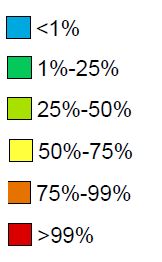
\includegraphics[width=0.6\textwidth]{images/legenda}
\caption{The range of colors used in the creation of a heat map. Defects inserted into the blue cells led to error events in a circuit in less than 1 \% of the simulations, \textit{i.e.}, for every 100 defects inserted into the cell, no more than one of them resulted in an error event. Analogous reasoning may be applied to the remaining colors.}
\label{figure:heatmap_caption}
\end{figure}

According to the range of colors presented in the Figure \ref{figure:heatmap_caption}, structural defects inserted into dark blue cells led to errors at the output signal(s) of a QCA structure in less than 1 \% of the simulations, \textit{i.e.}, for every 100 defects inserted into the cell, no more than one of them resulted in an error event at the outputs of the structure. Defects inserted into green colored cells led to errors in 1-25 \% of all simulations. Analogous reasoning may be applied to light green, yellow and orange colored cells complying with their respective percentage ranges indicated in the illustration. Defects inserted into red colored cells led to errors in more than 99 \% of all simulations in which the cells suffered under a defect.

It is important to highlight that the number of iterations, the probability model and the subgroup of parameters `Round Configuration' should be carefully set in order to ensure that the colors depicted in a heat map correspond to a realistic representation regarding to the correspondence between defective devices and error events. If the number of iterations is insufficient, wrong conclusions may be draw by analyzing the output heat map. For instance, suppose that a 28-cell structure undergoes defects simulation through sequential probability model, with all the four defect classes defined. Considering that, each cell should be made defective at least four times, so that defects from all the four classes may be inserted into each cell. Thus, a reasonable number of minimum iterations in a characterization round for that situation is four. For each iteration, 28 simulations are performed \textemdash since one cell is defective per simulation in the `Sequential' probability model \textemdash yielding a total of 72 simulations, which corresponds to a rate of 4 simulations/cell.

The Figures \ref{figure:heatmap_ex1} and \ref{figure:heatmap_ex2} depict some examples of real heat maps in order to better illustrate their meaning. The first figure refers to a NOT gate, while the second represents a majority gate. Since this section does not intend to analyze any results obtained from Error Analysis Module, the heat maps are depicted but not interpreted. Further information about results analysis may be found in the Sections \ref{section:Strategies_for_Robustness_Enhancement} and \ref{section:Results}.

\begin{figure}[H]
\center
\subfloat[A heatmap for a NOT gate tested against all structural defect classes with an uniform probability. \label{figure:heatmap_ex1}]{\includegraphics[width=0.40\textwidth]{images/heatmap_ex1}
}
\hfill
\subfloat[A heatmap for a majority gate tested against dopant structural defects with an uniform probability.\label{figure:heatmap_ex2}]{\includegraphics[width=0.45\textwidth]{images/heatmap_ex2}
}
\caption{Examples of heat maps.}
\label{figure:heatmap_examples}
\end{figure}

The heat maps are important visual resources that assist in the development of strategies for robustness enhancement for the QCA paradigm, since they allow in the identification of weak polarized regions within the structures. Since a weak region is identified, additional cells placement may be a good choice to ensure an extra polarization strength hence decreasing the likelihood of such cells to cause errors to the signal(s) at the output(s). In the next chapter, \ref{section:Strategies_for_Robustness_Enhancement}, there are further information about the heat map-based techniques applied in this work, by which the robustness of the QCA structures could be enhanced.